\chapter{Chimie de l'environnement et toxicologie}\label{ch:b3:environmental-toxicology}

Chaque fin d'été, les satellites photographient des volutes vertes qui
s'étendent sur de grands lacs~: des proliférations d'algues nourries par
le phosphate et le nitrate qui ruissellent des champs et sortent des
villes. Quand les algues meurent et coulent, leur décomposition consomme
le dioxygène des eaux profondes, et les poissons meurent. La chimie
explique chaque maillon de cette chaîne, et de bien d'autres~: pourquoi
certains gaz réchauffent la planète et d'autres non, pourquoi la pluie est
acide même dans un air propre, où aboutit un pesticide une fois pulvérisé,
et quelle quantité d'une substance il faut pour nuire. Ce chapitre
applique les équilibres, la cinétique et la spectroscopie à l'atmosphère,
aux eaux naturelles et aux sols, suit les polluants de l'un à l'autre, et
se termine par les grandeurs sur lesquelles reposent les évaluations des
risques.

\begin{recall}
Le volume de première année a couvert les équilibres acido-basiques, de
précipitation et de complexation, les diagrammes potentiel--pH, les
coefficients de partage, les temps de demi-vie, le danger, le risque et le
système SGH~; le volume scolaire, les \omterm{def:b3:environmental-toxicology:greenhouse}{gaz à effet de serre}~; le volume de
deuxième année, la loi de Henry, la force ionique, les statistiques, la
spectrométrie de masse et la spectrométrie atomique. Le
\cref{ch:b3:photochemistry} a traité la photochimie atmosphérique, le
\cref{ch:b3:group-theory-applied} et le
\cref{ch:b3:rovibrational-spectroscopy} l'activité infrarouge, et le
\cref{ch:b3:surfaces-catalysis} l'\omterm{def:b3:surfaces-catalysis:adsorption}{adsorption}.
\end{recall}

\begin{omfigure}
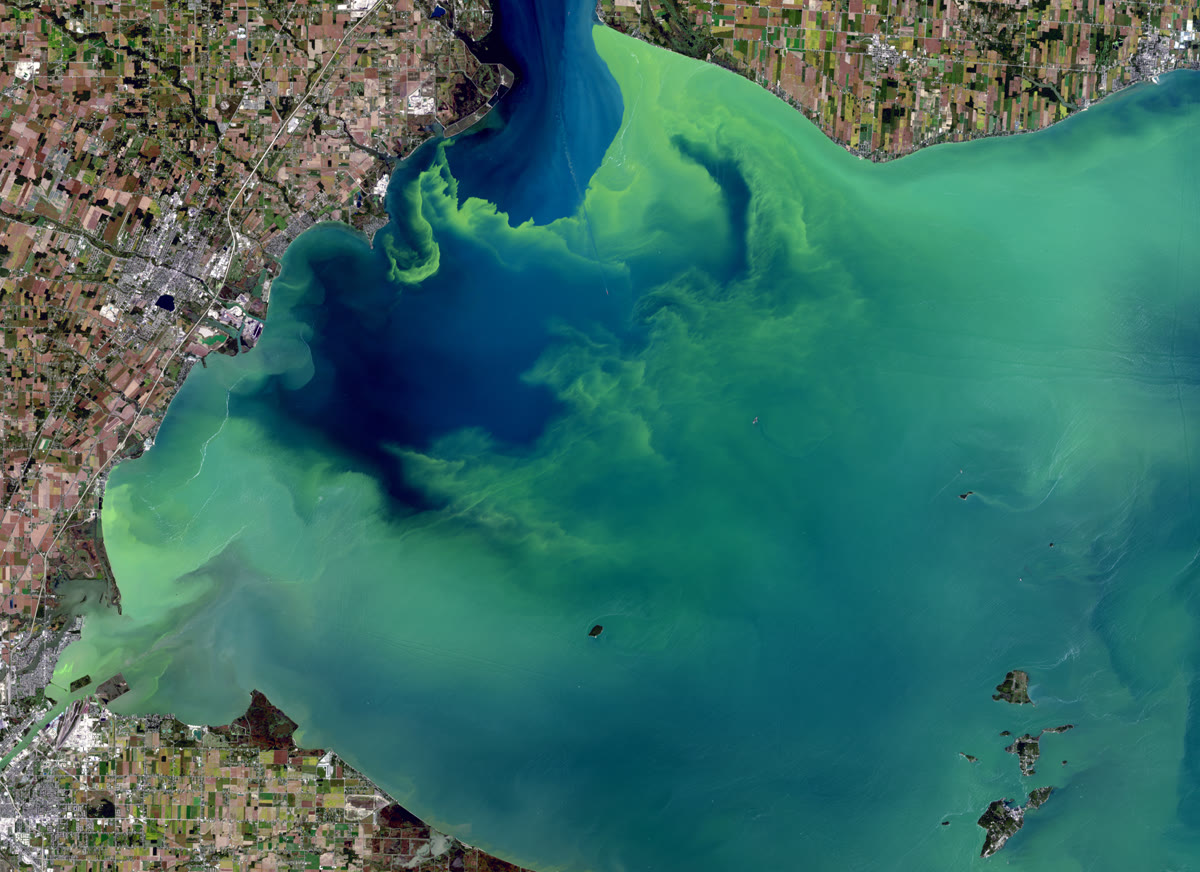
\includegraphics[width=0.62\linewidth]{images/book4/algal-bloom.jpg}

{\small Une prolifération d'algues sur un grand lac, vue par un satellite
d'observation de la Terre fin septembre~: les volutes vertes sont des
populations denses d'algues microscopiques nourries par les éléments
nutritifs des terres agricoles environnantes. Image~: USGS et NASA,
domaine public.}
\end{omfigure}

\section{L'atmosphère}

\begin{definition}[Gaz à effet de serre]\label{def:b3:environmental-toxicology:greenhouse}
Un \emph{gaz à effet de serre}\index{gaz a effet de serre@gaz à effet de serre} absorbe et émet le
rayonnement infrarouge aux longueurs d'onde du rayonnement émis par la
surface de la Terre, et réchauffe ainsi la basse atmosphère. Le
\emph{potentiel de réchauffement global}\index{potentiel de rechauffement global@potentiel de réchauffement global} (PRG) d'un gaz sur un
horizon de temps, en général 100 ans, est l'énergie qu'il piège après
l'émission d'un kilogramme, rapportée à celle d'un kilogramme de dioxyde
de carbone.
\end{definition}

Une molécule n'absorbe le rayonnement infrarouge que par des vibrations
qui modifient son moment dipolaire (\cref{ch:b3:group-theory-applied}). Le
diazote et le dioxygène, diatomiques homonucléaires, n'ont pas de telle
vibration et sont transparents~; l'argon n'a aucune vibration. Le dioxyde
de carbone, linéaire et apolaire, possède un mode de déformation actif en
infrarouge vers \qty{15}{\micro\metre}, au milieu de l'émission terrestre~; l'eau, le méthane
et le protoxyde d'azote absorbent à de nombreuses longueurs d'onde.

% ledger: atm:CO2.2025, atm:CH4.2025, atm:N2O.2025, gwp:CH4.fossil, gwp:CH4.nonfossil, gwp:N2O, life:CH4, life:N2O
En 2025, les fractions molaires moyennes mondiales étaient de \qty{425.6}{ppm} de dioxyde de carbone, \qty{1936}{ppb} de
méthane et \qty{338.9}{ppb} de protoxyde d'azote. Le méthane, éliminé par les radicaux hydroxyle avec une
durée de vie d'environ 12 ans, a un PRG à 100 ans de 27 à 30~; le protoxyde d'azote, détruit seulement dans
la stratosphère avec une durée de vie d'environ 109 ans, de 273. Le dioxyde
de carbone n'a pas de durée de vie unique~: une partie d'une émission reste
dans l'air pendant des siècles.

\begin{definition}[Polluants de l'air]\label{def:b3:environmental-toxicology:pollutants}
Les \emph{particules en suspension}\index{particules en suspension} sont les particules
solides et liquides en suspension dans l'air, classées selon leur diamètre
aérodynamique (les particules fines, de moins de \qty{2.5}{\micro\metre}, pénètrent profondément dans les poumons). Une \emph{pluie acide}\index{pluie acide} est une pluie
rendue plus acide qu'une pluie propre par les acides sulfurique et
nitrique formés à partir du dioxyde de soufre et des oxydes d'azote.
\end{definition}

\begin{proposition}[pH d'une pluie propre]\label{prop:b3:environmental-toxicology:rain-ph}
Une pluie en équilibre avec le dioxyde de carbone de l'air actuel, et avec
rien d'autre, a un pH d'environ 5.6.
\end{proposition}

\begin{proof}
% ledger: henry:CO2, pka4:H2CO3.1, pkw4:25C, const:atm
La loi de Henry donne $[\ce{CO2(aq)}] = K_Hp(\ce{CO2}) = \qty{3.4e-7}{mol.L^{-1}.Pa^{-1}} \times (425.6 \times 10^{-6} \times \qty{101325}{Pa}) = \qty{1.47e-5}{mol/L}$. L'électroneutralité
s'écrit $[\ce{H+}] = [\ce{HCO3-}] + 2[\ce{CO3^2-}] + [\ce{OH-}] \approx K_{a1}[\ce{CO2(aq)}]/[\ce{H+}] + K_w/[\ce{H+}]$, donc
$[\ce{H+}]^2 = K_{a1}[\ce{CO2(aq)}] + K_w = 10^{-6.35} \times \num{1.47e-5} + 10^{-14} = \num{6.6e-12}$~: $[\ce{H+}] = \qty{2.6e-6}{mol/L}$, pH 5.6.
\end{proof}

Le dioxyde de soufre issu de la combustion de combustibles soufrés et les
oxydes d'azote issus des combustions à haute température sont oxydés dans
l'air, par les radicaux hydroxyle et dans les gouttelettes des nuages, en
acides sulfurique et nitrique, qui abaissent le pH de la pluie à 4 et
au-dessous. La désulfuration des combustibles et l'élimination des oxydes
d'azote des gaz d'échappement (pots catalytiques, injection d'ammoniac dans
les centrales) ont largement résolu le problème là où elles ont été
appliquées. L'ozone au niveau du sol, formé quand la lumière solaire agit
sur les oxydes d'azote et les composés organiques volatils
(\cref{ch:b3:photochemistry}), et les particules fines restent les
principaux polluants de l'air pour la santé.

\section{Les eaux naturelles}

\begin{omfigure}
\begin{tikzpicture}
\begin{axis}[name=a, width=0.48\linewidth, height=5.4cm, xmin=4, xmax=13, ymin=0, ymax=1.02,
  axis lines=left, xlabel={pH}, ylabel={fraction du carbone dissous},
  tick label style={font=\scriptsize}, label style={font=\small}]
\addplot[color=omDef, thick] table[x=pH, y=a0] {figdata/out/bachelor-3-carbonate-system.dat};
\addplot[color=omMeth, thick] table[x=pH, y=a1] {figdata/out/bachelor-3-carbonate-system.dat};
\addplot[color=omThm, thick] table[x=pH, y=a2] {figdata/out/bachelor-3-carbonate-system.dat};
\node[font=\scriptsize, omDef] at (axis cs:4.9,0.85) {$\ce{CO2(aq)}$};
\node[font=\scriptsize, omMeth] at (axis cs:8.3,0.88) {$\ce{HCO3-}$};
\node[font=\scriptsize, omThm] at (axis cs:12.1,0.85) {$\ce{CO3^2-}$};
\draw[black!30, dashed] (axis cs:6.35,0) -- (axis cs:6.35,0.5) (axis cs:10.33,0) -- (axis cs:10.33,0.5);
\end{axis}
\begin{axis}[at={(a.east)}, anchor=west, xshift=1.4cm, width=0.48\linewidth, height=5.4cm,
  xmin=0, xmax=2000, ymin=5.2, ymax=6.2, axis lines=left,
  xlabel={$\ce{CO2}$ dans l'air / ppm}, ylabel={pH de la pluie},
  tick label style={font=\scriptsize}, label style={font=\small},
  scaled x ticks=false, xticklabel style={/pgf/number format/1000 sep={}}]
\addplot[color=omDef, thick] table[x=ppm, y=pH] {figdata/out/bachelor-3-carbonate-system-b.dat};
\draw[black!35, dashed] (axis cs:425.6,5.2) -- (axis cs:425.6,5.59);
\node[font=\scriptsize, anchor=west] at (axis cs:470,5.63) {aujourd'hui~: 5.6};
\end{axis}
\end{tikzpicture}

{\small À gauche~: répartition du carbone inorganique dissous entre ses
trois formes en fonction du pH à \qty{25}{\celsius}, avec des croisements à $\mathrm pK_{a1} = 6.35$ et $\mathrm pK_{a2} = 10.33$. À droite~: pH d'une pluie en
équilibre avec le seul dioxyde de carbone, en fonction de sa fraction
molaire dans l'air.}
\end{omfigure}

\begin{proposition}[Fractions des espèces carbonatées]\label{prop:b3:environmental-toxicology:carbonate-fractions}
Avec $C_T$ le carbone inorganique dissous total,
$[\ce{CO2(aq)}] = C_Th^2/D$, $[\ce{HCO3-}] = C_TK_{a1}h/D$, $[\ce{CO3^2-}] = C_TK_{a1}K_{a2}/D$, où $h = [\ce{H+}]$ et $D = h^2 + K_{a1}h + K_{a1}K_{a2}$.
\end{proposition}

\begin{proof}
D'après les deux constantes d'acidité,
\[
  [\ce{HCO3-}] = \frac{K_{a1}[\ce{CO2(aq)}]}{h}, \qquad [\ce{CO3^2-}] = \frac{K_{a2}[\ce{HCO3-}]}{h} = \frac{K_{a1}K_{a2}[\ce{CO2(aq)}]}{h^2}.
\]
Leur somme vaut $C_T = [\ce{CO2(aq)}]\,D/h^2$~; la division de chaque forme par $C_T$ donne les fractions.
\end{proof}

\begin{definition}[Alcalinité]\label{def:b3:environmental-toxicology:alkalinity}
L'\emph{alcalinité}\index{alcalinite@alcalinité} d'une eau est sa capacité à neutraliser un
acide fort, mesurée par titrage jusqu'au point d'équivalence de l'acide
carbonique (vers pH 4.5) et exprimée en moles de $\ce{H+}$ par litre.
\end{definition}

\begin{proposition}[Alcalinité carbonatée]\label{prop:b3:environmental-toxicology:alkalinity}
Dans une eau dont les bases sont les espèces carbonatées et l'hydroxyde,
$\mathrm{Alk} = [\ce{HCO3-}] + 2[\ce{CO3^2-}] + [\ce{OH-}] - [\ce{H+}]$~; elle est égale à l'excès des charges des cations de bases fortes
sur celles des anions d'acides forts, et ne varie pas lorsque du dioxyde de
carbone est échangé avec l'air.
\end{proposition}

\begin{proof}
Le titrage jusqu'au point d'équivalence de l'acide carbonique transforme chaque $\ce{HCO3-}$ en $\ce{CO2}$ (un $\ce{H+}$ chacun),
chaque $\ce{CO3^2-}$ en $\ce{CO2}$ (deux), chaque $\ce{OH-}$ en eau (un), tandis que les $\ce{H+}$ libres déjà présents
comptent en négatif~: c'est la somme annoncée. L'électroneutralité de
l'eau, avec
$\ce{Na+}$, $\ce{Ca^2+}$\dots{} et $\ce{Cl-}$, $\ce{SO4^2-}$\dots, se réarrange en la même somme, égale à $\sum z_i c_i$(cations) $-$ $\sum z_jc_j$(anions)
des électrolytes forts. Ajouter ou retirer du $\ce{CO2}$ ne modifie aucun de ces ions.
\end{proof}

\begin{definition}[Acidification des océans]\label{def:b3:environmental-toxicology:acidification}
L'\emph{acidification des océans}\index{acidification des oceans@acidification des océans} est la diminution du
pH de l'eau de mer à mesure qu'elle absorbe du dioxyde de carbone de l'air.
L'\emph{état de saturation}\index{etat de saturation@état de saturation} d'un minéral carbonaté vaut
$\Omega = [\ce{Ca^2+}][\ce{CO3^2-}]/K_{sp}$~: au-dessus de 1, le minéral peut se former~; au-dessous de 1, il tend à se dissoudre.
\end{definition}

Le dioxyde de carbone dissous transforme les ions carbonate en hydrogénocarbonate, $\ce{CO2 + CO3^2- + H2O -> 2HCO3-}$,
ce qui abaisse le pH et $\Omega$~: les coquilles et les squelettes coralliens deviennent plus difficiles à construire. (Dans
l'eau de mer, les constantes sont des constantes apparentes, mesurées dans
le milieu salin, et diffèrent des valeurs en eau douce de ce chapitre.)

\begin{definition}[Dureté de l'eau]\label{def:b3:environmental-toxicology:hardness}
La \emph{dureté}\index{durete de l'eau@dureté de l'eau} d'une eau est sa concentration totale en
ions calcium et magnésium, souvent exprimée par la masse de carbonate de
calcium contenant le même nombre de moles, en mg/L.
\end{definition}

\begin{definition}[Demande en oxygène]\label{def:b3:environmental-toxicology:oxygen-demand}
La \emph{demande biochimique en oxygène}\index{demande biochimique en oxygene@demande biochimique en oxygène} (DBO, ou BOD selon le
sigle anglais) d'une eau est la masse de dioxygène consommée par litre par
les micro-organismes qui oxydent sa matière organique dans l'obscurité,
pendant une durée donnée (cinq jours à \qty{20}{\celsius} pour la $\mathrm{BOD_5}$). Sa
\emph{demande chimique en oxygène}\index{demande chimique en oxygene@demande chimique en oxygène} (DCO, ou COD) est la masse de
dioxygène équivalente au dichromate consommé pour oxyder chimiquement sa
matière organique.
\end{definition}

\begin{proposition}[Courbe de DBO]\label{prop:b3:environmental-toxicology:bod}
Si la matière organique biodégradable est consommée selon une cinétique du
premier ordre de constante de vitesse $k$, le dioxygène utilisé au bout du temps $t$ vaut $\mathrm{BOD}_t = L_0(1 - \eu^{-kt})$, où $L_0$ est la DBO ultime.
\end{proposition}

\begin{proof}
La demande restante $L$ obéit à $\dd L/\dd t = -kL$, donc $L = L_0\eu^{-kt}$~; le dioxygène utilisé est ce qui a disparu,
$L_0 - L$.
\end{proof}

\begin{omfigure}
\begin{tikzpicture}
\begin{axis}[name=a, width=0.48\linewidth, height=5.2cm, xmin=0, xmax=30, ymin=0, ymax=270,
  axis lines=left, xlabel={temps / jours}, ylabel={DBO / \unit{mg.L^{-1}}},
  tick label style={font=\scriptsize}, label style={font=\small}]
\addplot[color=omDef, thick] table[x=t, y=bod] {figdata/out/bachelor-3-bod.dat};
\draw[black!35, dashed] (axis cs:0,250) -- (axis cs:30,250);
\draw[black!35, dashed] (axis cs:5,0) -- (axis cs:5,170.8);
\node[font=\scriptsize, anchor=west] at (axis cs:5.6,140) {$\mathrm{BOD_5}$};
\node[font=\scriptsize, anchor=north east] at (axis cs:30,246) {$L_0$};
\end{axis}
\begin{axis}[at={(a.east)}, anchor=west, xshift=1.4cm, width=0.48\linewidth, height=5.2cm,
  xmin=0, xmax=15, ymin=0, ymax=10, axis lines=left,
  xlabel={temps en aval / jours}, ylabel={$\ce{O2}$ dissous / \unit{mg.L^{-1}}},
  tick label style={font=\scriptsize}, label style={font=\small}]
\addplot[color=omThm, thick] table[x=t, y=O2] {figdata/out/bachelor-3-bod-b.dat};
\draw[black!35, dashed] (axis cs:0,9.1) -- (axis cs:15,9.1);
\node[font=\scriptsize, anchor=south east] at (axis cs:15,9.1) {saturation};
\node[font=\scriptsize, anchor=north] at (axis cs:2.4,6.3) {point critique};
\end{axis}
\end{tikzpicture}

{\small À gauche~: la DBO d'une eau usée modèle, $L_0 = \qty{250}{mg/L}$ et $k = \qty{0.23}{d^{-1}}$~: environ deux tiers de la
demande sont consommés en cinq jours. À droite~: le déficit en oxygène d'une
rivière en aval d'un rejet (modèle de Streeter--Phelps)~: la décomposition
de la charge organique consomme d'abord le dioxygène plus vite que l'air ne
le restaure, jusqu'à ce que le déficit culmine au bout d'environ 2.4 jours.}
\end{omfigure}

\begin{method}[Déterminer la DCO]\label{met:b3:environmental-toxicology:cod}
\begin{enumerate}
  \item Porter à reflux un volume mesuré d'échantillon avec un excès connu
        de dichromate de potassium en milieu sulfurique, avec du sulfate
        d'argent comme catalyseur et du sulfate de mercure(II) pour fixer
        les chlorures.
  \item Titrer le dichromate restant par le fer(II) en présence de
        ferroïne, et réaliser un blanc avec de l'eau pure.
  \item Le dichromate consommé, converti en masse équivalente de $\ce{O2}$ (un
        $\ce{Cr2O7^2-}$ capte six électrons, comme le feraient 1.5 $\ce{O2}$), divisé par le volume d'échantillon, donne la
        DCO en mg/L.
\end{enumerate}
\end{method}

\begin{definition}[Eutrophisation]\label{def:b3:environmental-toxicology:eutrophication}
L'\emph{eutrophisation}\index{eutrophisation} est l'enrichissement d'une
masse d'eau en éléments nutritifs, principalement le phosphore et l'azote,
qui conduit à une croissance excessive des algues et des plantes, puis à un
appauvrissement en oxygène lors de leur décomposition.
\end{definition}

\begin{omfigure}
\begin{tikzpicture}[font=\scriptsize, >=Stealth,
  box/.style={draw, rounded corners, align=center, fill=omMeth!10, inner sep=3pt, minimum height=8mm}]
  \node[box] (f) at (-4.3,1.2) {champs~: engrais,\\ fumier};
  \node[box] (t) at (-3.4,-0.4) {villes~: eaux usées,\\ lessives};
  \node[box] (a) at (0,2.1) {atmosphère~:\\ dépôts (N)};
  \node[box, fill=omDef!12, minimum width=3.2cm, minimum height=1.7cm] (l) at (0.6,0.4) {eau du lac~:\\ les algues croissent};
  \node[box, fill=black!8] (s) at (0.6,-1.6) {sédiment~: P stocké,\\ relargué en anoxie};
  \node[box] (o) at (4.0,0.4) {exutoire};
  \draw[->, thick] (f) -- node[above, sloped, pos=0.5] {ruissellement} (l);
  \draw[->, thick] (t) -- node[below, sloped] {N, P} (l);
  \draw[->, thick] (a) -- (l);
  \draw[->, thick] (l) -- node[left] {algues mortes} (s);
  \draw[->, thick, dashed] (s.east) to[bend right=30] node[right] {P} (l.south east);
  \draw[->, thick] (l) -- (o);
\end{tikzpicture}

{\small Flux d'éléments nutritifs vers un lac et en son sein. Le phosphore,
souvent l'élément limitant en eau douce, s'accumule dans le sédiment et
retourne dans l'eau quand le fond perd son oxygène, ce qui peut entretenir
des proliférations pendant des années après l'arrêt des apports.}
\end{omfigure}

Les algues absorbent le carbone, l'azote et le phosphore dans des
proportions à peu près constantes~; l'élément nutritif qui manque par
rapport à ces besoins limite leur croissance. Dans la plupart des lacs,
c'est le phosphore, ce qui explique qu'on ait retiré les phosphates des
lessives et des eaux usées traitées~; dans de nombreuses mers côtières,
c'est l'azote.

\begin{definition}[Spéciation]\label{def:b3:environmental-toxicology:speciation}
La \emph{spéciation chimique}\index{speciation chimique@spéciation chimique} d'un élément dans un
échantillon est la répartition de sa quantité entre ses formes
chimiques~: degrés d'oxydation, complexes, composés organométalliques,
espèces libres et liées.
\end{definition}

La toxicité dépend de la spéciation. Le mercure inorganique rejeté dans
l'eau est méthylé par les bactéries des sédiments en méthylmercure, qui
traverse les membranes, se lie au soufre des protéines et se concentre le
long des chaînes alimentaires~; l'arsenic est bien plus toxique sous forme
d'arsénite, As(III), que d'arséniate, As(V), et beaucoup moins sous les
formes organiques présentes dans les produits de la mer. Une concentration
totale seule renseigne peu.

\begin{method}[Spéciation d'un métal dans une eau]\label{met:b3:environmental-toxicology:speciation}
\begin{enumerate}
  \item Lister les ligands présents (hydroxyde, carbonate, chlorure,
        sulfate, matière organique) avec leurs concentrations et le pH.
  \item Écrire les constantes de complexation et le bilan de matière du
        métal, comme dans le volume de première année.
  \item Résoudre pour l'ion métallique libre, puis pour chaque complexe~;
        tracer les fractions en fonction du pH ou de la concentration d'un
        ligand.
  \item Comparer la forme toxique ou biodisponible (souvent l'ion libre)
        au total.
\end{enumerate}
\end{method}

\section{Sols et sédiments}

\begin{definition}[Sorption dans les sols]\label{def:b3:environmental-toxicology:soil}
La \emph{capacité d'échange cationique}\index{capacite d'echange cationique@capacité d'échange cationique} d'un sol est la
quantité de cations échangeables qu'il peut retenir par unité de masse,
sur les argiles et la matière organique. Le \emph{coefficient de distribution sol--eau}\index{coefficient de distribution sol--eau}
$K_d$ est le rapport de la concentration d'une substance
sorbée sur le sol (par kilogramme) à sa concentration dans l'eau
interstitielle (par litre)~; le \emph{coefficient de partage carbone organique--eau}\index{coefficient de partage carbone organique--eau}
vaut $K_{oc} = K_d/f_{oc}$, avec $f_{oc}$ la fraction massique de carbone organique.
\end{definition}

Les composés organiques neutres se sorbent principalement sur la matière organique du sol, si bien que $K_{oc}$ varie
beaucoup moins d'un sol à l'autre que $K_d$. Un composé de faible $K_d$ se déplace avec l'eau
et peut atteindre les eaux souterraines (lixiviation)~; un composé de $K_d$ élevé reste près de la surface,
lié à des particules que l'érosion peut entraîner vers les rivières et les
lacs.

\section{Devenir des polluants}

\begin{definition}[Coefficient de partage octanol--eau]\label{def:b3:environmental-toxicology:kow}
Le \emph{coefficient de partage octanol--eau}\index{coefficient de partage octanol--eau}
$K_{ow}$ d'une substance est le rapport de ses concentrations à l'équilibre
dans l'octan-1-ol et dans l'eau~; il mesure son affinité pour les tissus
graisseux et la matière organique.
\end{definition}

% ledger: logkow:DDT, logkow:benzene, logkow:atrazine, logkow:PCB153
Le benzène a $\log K_{ow} = 2.13$, l'herbicide atrazine 2.61, un PCB hexachloré 6.67 et
le DDT 6.91~: les deux derniers se dissolvent dans les graisses des dizaines
de millions de fois mieux que dans l'eau.

\begin{definition}[Bioaccumulation]\label{def:b3:environmental-toxicology:bio}
Le \emph{facteur de bioconcentration}\index{facteur de bioconcentration} (BCF) est le
rapport de la concentration dans un organisme à celle de l'eau environnante
en régime stationnaire, l'absorption se faisant à partir de l'eau seule. La
\emph{bioaccumulation}\index{bioaccumulation} est l'accumulation dans un
organisme par toutes les voies, alimentation comprise~; la
\emph{bioamplification}\index{bioamplification} est l'augmentation de la
concentration de la proie au prédateur le long d'une chaîne alimentaire.
\end{definition}

\begin{proposition}[BCF et $K_{ow}$]\label{prop:b3:environmental-toxicology:bcf-kow}
Pour les substances organiques neutres non métabolisées, $\log\mathrm{BCF}$ chez le poisson est
approximativement une fonction linéaire de $\log K_{ow}$, de pente voisine de 1, jusqu'à $\log K_{ow}$ voisin de 6~;
au-delà, l'absorption ralentit et la relation plafonne (régressions
empiriques).
\admitted
\end{proposition}

\begin{definition}[Polluants organiques persistants]\label{def:b3:environmental-toxicology:pop}
Un \emph{polluant organique persistant}\index{polluant organique persistant} est une
substance organique qui résiste à la dégradation, se bioaccumule, est
toxique et est transportée loin de ses sources, comme le DDT, les PCB et
les dioxines.
\end{definition}

\begin{proposition}[Répartition à l'équilibre entre compartiments]\label{prop:b3:environmental-toxicology:level-one}
Une masse $M$ d'une substance répartie à l'équilibre (modèle de «~niveau~I~») entre l'eau
(volume $V_w$), l'air ($V_a$), les solides du sédiment ($m_s$) et les poissons ($m_f$) a pour concentration dans l'eau
$C_w = M/(V_w + K_{aw}V_a + K_{sw}m_s + K_{fw}m_f)$, où les $K$ sont les coefficients de partage par rapport à
l'eau~; la masse dans chaque compartiment est son terme multiplié par $C_w$.
\end{proposition}

\begin{proof}
À l'équilibre, $C_a = K_{aw}C_w$, $C_s = K_{sw}C_w$ (par kilogramme), $C_f = K_{fw}C_w$. Le bilan de matière s'écrit
$M = C_wV_w + C_aV_a + C_sm_s + C_fm_f = C_w(V_w + K_{aw}V_a + K_{sw}m_s + K_{fw}m_f)$~; la division donne $C_w$.
\end{proof}

\begin{omfigure}
\begin{tikzpicture}[font=\scriptsize, >=Stealth,
  comp/.style={draw, rounded corners, align=center, minimum width=2.6cm, minimum height=1.0cm}]
  \node[comp, fill=omDef!8] (air) at (0,2.2) {air\\ $C_a = K_{aw}C_w$};
  \node[comp, fill=omDef!25] (w) at (0,0.6) {eau\\ $C_w$};
  \node[comp, fill=black!10] (sed) at (0,-1.0) {sédiment\\ $C_s = K_{sw}C_w$};
  \node[comp, fill=omMeth!15] (fish) at (3.6,0.6) {poissons\\ $C_f = K_{fw}C_w$};
  \node[comp, fill=omProp!15] (soil) at (-3.6,0.6) {sol\\ $C_{soil} = K_dC_w$};
  \draw[<->, thick] (air) -- (w); \draw[<->, thick] (w) -- (sed);
  \draw[<->, thick] (w) -- (fish); \draw[<->, thick] (w) -- (soil);
\end{tikzpicture}

{\small Compartiments d'un modèle à l'équilibre (niveau~I)~: chaque
compartiment est en équilibre avec l'eau, sa concentration étant fixée par
un coefficient de partage. La substance s'accumule là où le produit de la
capacité par le volume (ou la masse) est le plus grand, souvent le sédiment
ou le sol pour un composé hydrophobe.}
\end{omfigure}

\section{Toxicologie et réglementation}

\begin{definition}[Dose--réponse]\label{def:b3:environmental-toxicology:dose}
Une \emph{relation dose--réponse}\index{relation dose--reponse@relation dose--réponse} relie la
dose d'une substance à l'ampleur ou à la fréquence d'un effet. La \emph{dose létale médiane}\index{dose letale mediane@dose létale médiane} $\mathrm{LD_{50}}$ (DL50 en français) tue la moitié d'une population d'essai~; la
\emph{concentration efficace médiane}\index{concentration efficace mediane@concentration efficace médiane} $\mathrm{EC_{50}}$
(CE50) provoque un effet donné chez la moitié. La \emph{dose sans effet nocif observé}\index{dose sans effet nocif observe@dose sans effet nocif observé} (NOAEL) est la plus forte dose
testée sans effet nocif, la \emph{dose minimale avec effet nocif observé}\index{dose minimale avec effet nocif observe@dose minimale avec effet nocif observé} (LOAEL) la plus faible dose
testée qui en produit un.
\end{definition}

\begin{proposition}[Modèle log-logistique]\label{prop:b3:environmental-toxicology:dose-response}
Dans le modèle log-logistique $f(d) = 1/\bigl(1 + (D_{50}/d)^n\bigr)$, la réponse vaut un demi pour $d = D_{50}$, et $n$
mesure la raideur~: le rapport des doses entre les réponses de 10\,\% et de 90\,\% vaut $81^{1/n}$.
\end{proposition}

\begin{proof}
Pour $d = D_{50}$, $f = 1/2$. $f = 0.1$ exige $(D_{50}/d)^n = 9$, $f = 0.9$ exige $(D_{50}/d)^n = 1/9$~; le rapport des deux doses
vaut $(9 \times 9)^{1/n} = 81^{1/n}$.
\end{proof}

\begin{omfigure}
\begin{tikzpicture}
\begin{axis}[width=0.72\linewidth, height=5.4cm, xmode=log, xmin=3, xmax=3200, ymin=0, ymax=1.02,
  axis lines=left, xlabel={dose / \unit{mg.kg^{-1}}}, ylabel={fraction de répondants},
  tick label style={font=\scriptsize}, label style={font=\small}]
\addplot[color=omDef, thick] table[x=d, y=n2] {figdata/out/bachelor-3-dose-response.dat};
\addplot[color=omThm, thick] table[x=d, y=n6] {figdata/out/bachelor-3-dose-response.dat};
\addplot[only marks, mark=*, mark size=1.6pt, omThm] table[x=d, y=r] {figdata/out/bachelor-3-dose-response-b.dat};
\draw[black!35, dashed] (axis cs:200,0) -- (axis cs:200,0.5) -- (axis cs:3,0.5);
\node[font=\scriptsize, anchor=north west] at (axis cs:200,0.48) {$D_{50}$};
\node[font=\scriptsize, omThm, anchor=south east, inner sep=1pt] (noael) at (axis cs:60,0.09) {NOAEL};
\draw[omThm] (noael.south east) -- (axis cs:78,0.012);
\node[font=\scriptsize, omThm, anchor=west] at (axis cs:165,0.2) {LOAEL};
\node[font=\scriptsize, omDef, anchor=east] at (axis cs:60,0.25) {$n = 2$};
\node[font=\scriptsize, omThm, anchor=east] at (axis cs:185,0.8) {$n = 6$};
\end{axis}
\end{tikzpicture}

{\small Courbes dose--réponse log-logistiques de même dose médiane
(\qty{200}{mg/kg}, modèle) et de deux raideurs. Les points représentent une
étude à cinq doses pour la courbe la plus raide~: avec une réponse de
5\,\% comme critère d'effet nocif, la NOAEL vaut \qty{80}{mg/kg} et la
LOAEL \qty{160}{mg/kg}~; toutes deux dépendent des doses choisies.}
\end{omfigure}

\begin{definition}[Toxicité aiguë et chronique]\label{def:b3:environmental-toxicology:toxicity}
La \emph{toxicité aiguë}\index{toxicite aigue@toxicité aiguë} est le dommage causé par une exposition
unique ou des expositions rapprochées dans le temps~; la \emph{toxicité chronique}\index{toxicite chronique@toxicité chronique},
celui causé par une exposition répétée ou continue sur une longue partie
de la vie.
\end{definition}

% ledger: ld50:NaCl, ld50:caffeine, ld50:nicotine
La toxicité est une affaire de dose~: la $\mathrm{LD_{50}}$ par voie orale chez le rat vaut environ \qty{3000}{mg/kg} pour le chlorure de sodium,
\qty{192}{mg/kg} pour la caféine et \qty{188}{mg/kg} pour la nicotine dans le même type de source. Pour la plupart des effets, il
existe une dose seuil en dessous de laquelle l'organisme fait face~; pour
les cancérogènes génotoxiques, on n'en suppose aucune, et l'exposition est
maintenue aussi basse que raisonnablement possible.

\begin{definition}[Écotoxicologie]\label{def:b3:environmental-toxicology:ecotoxicology}
L'\emph{écotoxicologie}\index{ecotoxicologie@écotoxicologie} étudie les effets des substances sur
les organismes au sein des écosystèmes. La \emph{concentration prédite sans effet}\index{concentration predite sans effet@concentration prédite sans effet} (PNEC) est la plus faible
concentration à effet ou sans effet issue d'essais sur des espèces
représentatives, divisée par un facteur d'évaluation qui couvre
l'incertitude~; la \emph{concentration environnementale prédite}\index{concentration environnementale predite@concentration environnementale prédite}
(PEC) est la concentration attendue d'après les usages et le devenir de la
substance~; le \emph{quotient de risque}\index{quotient de risque} est le rapport PEC/PNEC.
\end{definition}

\begin{proposition}[Quotient de risque]\label{prop:b3:environmental-toxicology:risk-quotient}
Un \omterm{def:b3:environmental-toxicology:ecotoxicology}{quotient de risque} inférieur à 1 n'indique aucune préoccupation pour le
compartiment évalué~; supérieur à 1, un risque qui appelle des données
affinées ou des mesures de réduction de l'exposition.
\end{proposition}

\begin{proof}[Par définition]
La PNEC est fixée, grâce à son facteur d'évaluation, au-dessous des
concentrations auxquelles des effets ont été observés~; une concentration
attendue inférieure n'est donc pas censée causer d'effets, et une
concentration supérieure l'est.
\end{proof}

\begin{method}[Une évaluation du risque environnemental]\label{met:b3:environmental-toxicology:risk}
\begin{enumerate}
  \item Danger~: réunir les données de toxicité pour les algues, les invertébrés et les poissons (valeurs aiguës
        $\mathrm{EC_{50}}$, NOEC chroniques)~; retenir la plus faible~; la diviser par le facteur d'évaluation (plus grand quand
        seules des données aiguës existent) pour obtenir la PNEC.
  \item Exposition~: à partir des quantités utilisées et du devenir
        (partage, dégradation), calculer la PEC dans chaque compartiment, ou
        la mesurer.
  \item Risque~: calculer PEC/PNEC~; si le rapport dépasse 1, affiner les
        données ou réduire l'exposition, et recommencer.
\end{enumerate}
\end{method}

\begin{definition}[Valeur limite d'exposition professionnelle]\label{def:b3:environmental-toxicology:oel}
Une \emph{valeur limite d'exposition professionnelle}\index{valeur limite d'exposition professionnelle} est la
concentration d'une substance dans l'air d'un lieu de travail que les
travailleurs peuvent respirer, en moyenne sur une journée de travail (ou
sur 15 minutes pour les valeurs à court terme), sans effet nocif attendu.
\end{definition}

Les nouvelles substances chimiques mises sur un marché en quantité doivent
être enregistrées avec un dossier de leurs propriétés, de leurs dangers et
de leurs usages~; les plus dangereuses peuvent être restreintes ou
autorisées seulement pour certains usages.

\begin{inthelab}[Mesurer la $\mathrm{BOD_5}$]
Un échantillon est dilué par une eau de dilution aérée contenant des
éléments nutritifs et un ensemencement bactérien, de sorte qu'une bonne
partie, mais pas la totalité, du dioxygène soit consommée. Deux flacons
bouchés sont remplis à ras bord~: le dioxygène dissous de l'un est mesuré
immédiatement avec une électrode à oxygène, celui de l'autre après cinq
jours dans l'obscurité à
\qty{20}{\celsius}. La différence, multipliée par le facteur de dilution et corrigée de l'ensemencement, donne la
$\mathrm{BOD_5}$.
\end{inthelab}

\begin{safety}{\ghs[0.62cm]{GHS03}\ghs[0.62cm]{GHS05}\ghs[0.62cm]{GHS06}\ghs[0.62cm]{GHS08}\ghs[0.62cm]{GHS09}}
% ledger: ghs:K2Cr2O7, ghs4:HgSO4
Les réactifs de la DCO~: le dichromate de potassium est un comburant, peut
provoquer le cancer et des anomalies génétiques, est corrosif et
sensibilisant~; le sulfate de mercure(II) est mortel par ingestion, par
inhalation ou par contact cutané et très toxique pour les organismes
aquatiques. Tous deux s'utilisent en tubes scellés, et les tubes usagés
vont aux déchets dangereux.
\end{safety}

\begin{history}[Un livre et une baie]
En 1962, le \textit{Printemps silencieux} de Rachel Carson décrivit le déclin des oiseaux empoisonnés par
le DDT et d'autres pesticides concentrés le long des chaînes alimentaires,
et lança la réglementation environnementale moderne. Quelques années plus
tôt, en 1956, une maladie du système nerveux fut reconnue chez les
habitants de la baie de Minamata~: une usine chimique avait rejeté du
méthylmercure, formé à partir de son catalyseur au mercure, qui
s'accumulait dans les poissons que mangeaient les habitants.
\end{history}

\section{Exercices}

\begin{exercise}[$\star$]\label{exo:b3:environmental-toxicology:1}
Pourquoi $\ce{N2}$, $\ce{O2}$ et Ar n'absorbent-ils pas dans l'infrarouge, et quelle vibration de $\ce{CO2}$ en fait un
\omterm{def:b3:environmental-toxicology:greenhouse}{gaz à effet de serre}~?
\end{exercise}

\begin{exercise}[$\star$]\label{exo:b3:environmental-toxicology:2}
De quel facteur $[\ce{H+}]$ varie-t-il quand le pH de l'eau de mer diminue de 0.1~?
\end{exercise}

\begin{exercise}[$\star$]\label{exo:b3:environmental-toxicology:3}
Une eau contient \qty{2.0}{mmol/L} de $\ce{Ca^2+}$ et \qty{0.50}{mmol/L} de $\ce{Mg^2+}$. Donner sa \omterm{def:b3:environmental-toxicology:hardness}{dureté} en mg de $\ce{CaCO3}$ par litre.
\end{exercise}

\begin{exercise}[$\star$]\label{exo:b3:environmental-toxicology:4}
Les algues absorbent C, N et P dans le rapport molaire $106 : 16 : 1$ (données de l'exercice). Une eau de lac
contient \qty{0.60}{mg/L} d'azote nitrique et \qty{0.010}{mg/L} de phosphore phosphaté. Quel élément nutritif limite
la croissance~?
\end{exercise}

\begin{exercise}[$\star\star$]\label{exo:b3:environmental-toxicology:5}
Une $\mathrm{BOD_5}$ de \qty{170}{mg/L} est mesurée sur une eau usée avec $k = \qty{0.23}{d^{-1}}$. Estimer sa DBO ultime.
\end{exercise}

\begin{exercise}[$\star\star$]\label{exo:b3:environmental-toxicology:6}
Un échantillon d'eau de \qty{100.0}{mL} exige \qty{4.40}{mL} d'acide chlorhydrique à \qty{0.0200}{mol/L} pour atteindre pH 4.5. Calculer son
\omterm{def:b3:environmental-toxicology:alkalinity}{alcalinité} et, en supposant qu'elle est entièrement due à l'hydrogénocarbonate, la concentration de celui-ci en mg/L.
\end{exercise}

\begin{exercise}[$\star\star$]\label{exo:b3:environmental-toxicology:7}
Un sol a $f_{oc} = 0.020$~; un pesticide a $K_{oc} = \qty{300}{L/kg}$ (données de l'exercice). Calculer $K_d$ et la
fraction du pesticide sorbée dans un sol comportant \qty{1.5}{kg} de solide pour \qty{0.30}{L} d'eau interstitielle.
\end{exercise}

\begin{exercise}[$\star\star$]\label{exo:b3:environmental-toxicology:8}
Avec $\log\mathrm{BCF} = 0.85\log K_{ow} - 0.70$ (une régression empirique, données de l'exercice), estimer le BCF du
benzène et d'un PCB hexachloré, et commenter.
\end{exercise}

\begin{exercise}[$\star\star$]\label{exo:b3:environmental-toxicology:9}
Exprimer la $\mathrm{LD_{50}}$ orale de la caféine chez le rat en masse pour un adulte de \qty{70}{kg} et en tasses de café de
\qty{90}{mg} chacune (une extrapolation naïve, données de l'exercice). Pourquoi une telle extrapolation n'est-elle qu'indicative~?
\end{exercise}

\begin{exercise}[$\star\star\star$]\label{exo:b3:environmental-toxicology:10}
Une substance a une $\mathrm{EC_{50}}$ à 48 heures de \qty{0.50}{mg/L} pour les daphnies, une $\mathrm{EC_{50}}$ à 72 heures de \qty{1.2}{mg/L} pour les algues
et une $\mathrm{LC_{50}}$ à 96 heures de \qty{2.0}{mg/L} pour les poissons, toutes aiguës, et un facteur d'évaluation de 1000 s'applique
(données de l'exercice). Calculer la PNEC, et le \omterm{def:b3:environmental-toxicology:ecotoxicology}{quotient de risque} pour une PEC de \qty{0.20}{\micro g/L}.
\end{exercise}

\begin{exercise}[$\star\star\star$]\label{exo:b3:environmental-toxicology:11}
Un oiseau piscivore mange des poissons contenant \qty{0.30}{mg/kg} d'un polluant persistant~; les poissons mangent
du plancton à \qty{0.015}{mg/kg}~; l'eau en contient \qty{2.0}{ng/L}. Calculer les \omterm{def:b3:environmental-toxicology:bio}{facteurs de bioconcentration} et de
\omterm{def:b3:environmental-toxicology:bio}{bioamplification} le long de la chaîne si la graisse de l'oiseau en contient \qty{6.0}{mg/kg} (données de
l'exercice).
\end{exercise}

\begin{exercise}[$\star\star\star$]\label{exo:b3:environmental-toxicology:12}
Une centrale électrique émet \qty{1000}{t} de $\ce{SO2}$ par an. Calculer la masse d'acide sulfurique qu'elle peut former,
et le volume de pluie qu'elle amènerait à pH 4.0 si tout tombait sous forme de pluie (négliger les autres
acides et bases).
\end{exercise}

\section{Problème~: un pesticide dans un lac}

\begin{problem}[{Problème du week-end --- un pesticide dans un lac~: son
partage entre le sédiment et les poissons, un bilan de matière à
l'équilibre, sa dégradation sur un an, et le quotient de risque pour les
organismes du lac}]
\label{pb:b3:environmental-toxicology:1}
Données du problème. Un lac contient $\qty{1.0e9}{L}$ d'eau sous $\qty{1.0e12}{L}$ d'air (la couche de mélange au-dessus),
avec $\qty{1.0e8}{kg}$ de solides de sédiment actifs ($f_{oc} = 0.040$) et $\qty{1.0e4}{kg}$ de poissons (fraction lipidique 0.048).
Un pesticide a $\log K_{ow} = 4.0$, un coefficient de partage air--eau $K_{aw} = \num{1.0e-4}$, et $K_{oc} = 0.41\,K_{ow}$~;
$K_{fw}$ = fraction lipidique $\times K_{ow}$. 100 kg en parviennent au lac. Sa demi-vie dans le lac est de 60 jours.
L'essai chronique le plus sensible donne une NOEC de \qty{50}{\micro g/L}, avec un facteur d'évaluation de 10~;
les poissons destinés à la consommation humaine ne doivent pas dépasser \qty{1.0}{mg/kg}.

\medskip\noindent\textbf{Partie I --- Coefficients de partage.}
\begin{enumerate}
  \item Que dit $\log K_{ow} = 4.0$ du pesticide~?
  \item Calculer $K_{oc}$ et le coefficient sédiment--eau $K_{sw}$.
  \item Calculer le coefficient poisson--eau $K_{fw}$.
  \item Le pesticide est-il volatil à partir de l'eau~? Utiliser $K_{aw}$.
  \item Pourquoi est-ce le carbone organique, et non la matière minérale,
        qui gouverne sa sorption~?
  \item Quel compartiment devrait en contenir la plus grande part~?
\end{enumerate}

\medskip\noindent\textbf{Partie II --- Bilan de matière à l'équilibre.}
\begin{enumerate}[resume]
  \item Calculer les termes de capacité $V_w$, $K_{aw}V_a$, $K_{sw}m_s$ et $K_{fw}m_f$.
  \item Calculer la concentration dans l'eau.
  \item Calculer la masse dans chaque compartiment.
  \item Calculer les concentrations dans l'air, le sédiment et les
        poissons.
  \item Quelle hypothèse du modèle est la moins réaliste~?
  \item Comment la dégradation modifierait-elle le tableau (modèles de
        niveaux~II et III)~?
\end{enumerate}

\medskip\noindent\textbf{Partie III --- Dégradation.}
\begin{enumerate}[resume]
  \item Calculer la constante de vitesse du premier ordre.
  \item Calculer la fraction restante au bout d'un an.
  \item Calculer la concentration dans l'eau au bout d'un an.
  \item Pourquoi le sédiment peut-il retenir le pesticide plus longtemps
        que ne le suggère la demi-vie~?
  \item Qu'est-ce qui rend un pesticide persistant~?
\end{enumerate}

\medskip\noindent\textbf{Partie IV --- Le risque.}
\begin{enumerate}[resume]
  \item Calculer la PNEC.
  \item Prendre la concentration initiale dans l'eau comme PEC~: calculer le
        \omterm{def:b3:environmental-toxicology:ecotoxicology}{quotient de risque}.
  \item Conclure pour les organismes du lac.
  \item Comparer la concentration dans les poissons au seuil de
        consommation.
  \item Que faudrait-il mesurer ensuite, et où~?
  \item Quelles mesures abaisseraient la PEC~?
  \item Pourquoi le facteur d'évaluation compte-t-il autant~?
  \item Énoncer le résultat~: le \omterm{def:b3:environmental-toxicology:ecotoxicology}{quotient de risque} PEC/PNEC.
\end{enumerate}
\end{problem}
